% !TEX TS-program = pdflatex
\documentclass[11pt]{article}

% -------------------- Packages --------------------
\usepackage[a4paper,margin=1in]{geometry}
\usepackage{amsmath,amssymb}
\usepackage[T1]{fontenc}
\usepackage{lmodern}
\usepackage{xcolor}
\usepackage{tcolorbox}
\tcbuselibrary{skins,breakable}
\usepackage{enumitem}
\usepackage{hyperref}
\usepackage{tikz}
\usetikzlibrary{calc,angles,quotes}

\pagestyle{empty}

% -------------------- Dark Theme Colors --------------------
\definecolor{bg}{HTML}{000000}
\definecolor{pairbg}{HTML}{121212}
\definecolor{solbg}{HTML}{0A0A0A}
\definecolor{border}{HTML}{2A2A2A}
\definecolor{text}{HTML}{FFFFFF}
\definecolor{muted}{HTML}{C9CDD3}
\definecolor{gold}{HTML}{FFD700}
\definecolor{green}{HTML}{4ADE80}
\definecolor{cyan}{HTML}{38BDF8}

\pagecolor{bg}
\color{text}

\hypersetup{
  colorlinks=true,
  linkcolor=cyan,
  urlcolor=cyan
}

\setlength{\parindent}{0pt}
\setlength{\parskip}{10pt}

\setlist[itemize]{left=1.4em,itemsep=6pt,topsep=6pt}
\setlist[enumerate]{left=1.6em,itemsep=4pt,topsep=4pt}

% -------------------- tcolorbox Base --------------------
\tcbset{
  enhanced,
  breakable,
  arc=12pt,
  boxrule=0.8pt,
  left=16pt,right=16pt,top=12pt,bottom=12pt
}

\newtcolorbox{QAPair}[1]{%
  colback=pairbg,
  colbacklower=solbg,
  colframe=border,
  coltext=text,
  title=\textcolor{gold}{\bfseries #1},
  fonttitle=\bfseries,
  coltitle=text,
  segmentation style={draw=border, dashed, line width=0.6pt},
}

\newtcolorbox{QuickBox}{%
  colback=pairbg,
  colframe=cyan,
  coltext=text,
  fontupper=\color{text},
  borderline north={4pt}{0pt}{cyan},
  arc=14pt,
  boxrule=0.8pt
}

% Helper for step headings
\newcommand{\Step}[1]{\textcolor{muted}{\textbf{Step #1:}}}

% -------------------- TikZ styles --------------------
\tikzset{
  fig/.style={draw=cyan, line width=1.1pt},
  dim/.style={text=muted, font=\small},
  ang/.style={text=gold, font=\small},
  lbl/.style={text=text, font=\small},
  dot/.style={circle, fill=cyan, inner sep=1.2pt}
}

% ============================================================
\begin{document}

\begin{center}
{\LARGE\bfseries \textcolor{gold}{Exercise 9.2 --- Solutions}}\\[-2pt]
\end{center}

\begin{QuickBox}
{\color{cyan}\bfseries Quick facts (Similarity)}\par\medskip
\begin{itemize}
\item \textbf{AA criterion:} If two angles of one triangle equal two angles of another, the triangles are similar.
\item \textbf{SAS criterion:} If an included angle is equal and the two surrounding sides are in the same ratio, triangles are similar.
\item \textbf{SSS criterion:} If all three corresponding sides are in the same ratio, triangles are similar.
\item \textbf{Parallel line idea:} If a line is drawn parallel to one side of a triangle, it makes a smaller triangle similar to the whole triangle.
\item \textbf{Magnification (lens):} $\displaystyle m=\frac{\text{image size}}{\text{object size}}=\left|\frac{v}{u}\right|$.
\end{itemize}
\end{QuickBox}

% ============================================================
% Q1
\begin{QAPair}{Question 1: Which pairs of figures are similar?}
\textcolor{gold}{\bfseries Answer (final):}
\[
\boxed{\text{Similar pairs are (i), (ii), (iv), (vi), (vii). \quad Not similar: (iii), (v).}}
\]

\textcolor{muted}{(Diagrams are not to scale; they only show the given measures/angles.)}

\begin{center}
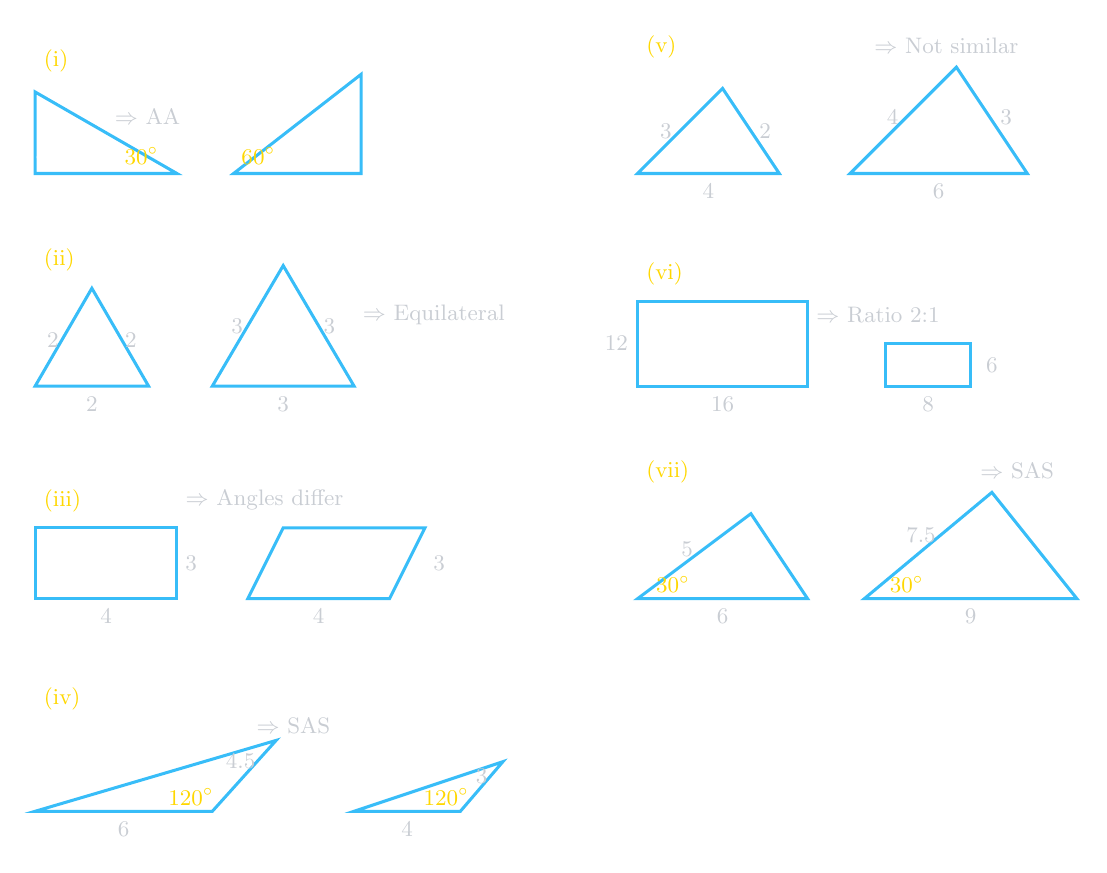
\begin{tikzpicture}[scale=0.9, transform shape]
    % --- COLUMN 1 ---
    
    % (i)
    \begin{scope}[shift={(0,0)}]
        \node[ang, anchor=south west] at (0,1.3) {(i)};
        \draw[fig] (0,0)--(2.0,0)--(0,1.15)--cycle;
        \node[lbl] at (0.25,0.2) {$90^\circ$};
        \node[ang] at (1.5,0.25) {$30^\circ$};
        
        \draw[fig] (2.8,0)--(4.6,0)--(4.6,1.4)--cycle;
        \node[lbl] at (4.35,0.2) {$90^\circ$};
        \node[ang] at (3.15,0.25) {$60^\circ$};
        \node[dim, anchor=west] at (1.0,0.8) {$\Rightarrow$ AA};
    \end{scope}

    % (ii)
    \begin{scope}[shift={(0,-3)}]
        \node[ang, anchor=south west] at (0,1.5) {(ii)};
        \draw[fig] (0,0)--(1.6,0)--(0.8,1.38)--cycle;
        \node[dim] at (0.8,-0.25) {$2$};
        \node[dim] at (0.25,0.65) {$2$};
        \node[dim] at (1.35,0.65) {$2$};

        \draw[fig] (2.5,0)--(4.5,0)--(3.5,1.7)--cycle;
        \node[dim] at (3.5,-0.25) {$3$};
        \node[dim] at (2.85,0.85) {$3$};
        \node[dim] at (4.15,0.85) {$3$};
        \node[dim, anchor=west] at (4.5,1.0) {$\Rightarrow$ Equilateral};
    \end{scope}

    % (iii)
    \begin{scope}[shift={(0,-6)}]
        \node[ang, anchor=south west] at (0,1.1) {(iii)};
        \draw[fig] (0,0)--(2.0,0)--(2.0,1.0)--(0,1.0)--cycle;
        \node[dim] at (1.0,-0.25) {$4$};
        \node[dim] at (2.2,0.5) {$3$};

        \draw[fig] (3.0,0)--(5.0,0)--(5.5,1.0)--(3.5,1.0)--cycle;
        \node[dim] at (4.0,-0.25) {$4$};
        \node[dim] at (5.7,0.5) {$3$};
        \node[dim, anchor=west] at (2.0,1.4) {$\Rightarrow$ Angles differ};
    \end{scope}

    % (iv)
    \begin{scope}[shift={(0,-9)}]
        \node[ang, anchor=south west] at (0,1.3) {(iv)};
        \draw[fig] (0,0)--(2.5,0)--(3.4,1.0)--cycle;
        \node[ang] at (2.2,0.2) {$120^\circ$};
        \node[dim] at (1.25,-0.25) {$6$};
        \node[dim] at (2.9,0.7) {$4.5$};

        \draw[fig] (4.5,0)--(6.0,0)--(6.6,0.7)--cycle;
        \node[ang] at (5.8,0.2) {$120^\circ$};
        \node[dim] at (5.25,-0.25) {$4$};
        \node[dim] at (6.3,0.5) {$3$};
        \node[dim, anchor=west] at (3.0,1.2) {$\Rightarrow$ SAS};
    \end{scope}


    % --- COLUMN 2 ---
    
    % (v)
    \begin{scope}[shift={(8.5,0)}]
        \node[ang, anchor=south west] at (0,1.5) {(v)};
        \draw[fig] (0,0)--(2.0,0)--(1.2,1.2)--cycle;
        \node[dim] at (1.0,-0.25) {$4$};
        \node[dim] at (1.8,0.6) {$2$};
        \node[dim] at (0.4,0.6) {$3$};

        \draw[fig] (3.0,0)--(5.5,0)--(4.5,1.5)--cycle;
        \node[dim] at (4.25,-0.25) {$6$};
        \node[dim] at (5.2,0.8) {$3$};
        \node[dim] at (3.6,0.8) {$4$};
        \node[dim, anchor=east] at (5.5,1.8) {$\Rightarrow$ Not similar};
    \end{scope}

    % (vi)
    \begin{scope}[shift={(8.5,-3)}]
        \node[ang, anchor=south west] at (0,1.3) {(vi)};
        \draw[fig] (0,0)--(2.4,0)--(2.4,1.2)--(0,1.2)--cycle;
        \node[dim] at (1.2,-0.25) {$16$};
        \node[dim] at (-0.3,0.6) {$12$};

        \draw[fig] (3.5,0)--(4.7,0)--(4.7,0.6)--(3.5,0.6)--cycle;
        \node[dim] at (4.1,-0.25) {$8$};
        \node[dim] at (5.0,0.3) {$6$};
        \node[dim, anchor=west] at (2.4,1.0) {$\Rightarrow$ Ratio 2:1};
    \end{scope}

    % (vii)
    \begin{scope}[shift={(8.5,-6)}]
        \node[ang, anchor=south west] at (0,1.5) {(vii)};
        \draw[fig] (0,0)--(2.4,0)--(1.6,1.2)--cycle;
        \node[ang] at (0.5,0.2) {$30^\circ$};
        \node[dim] at (1.2,-0.25) {$6$};
        \node[dim] at (0.7,0.7) {$5$};

        \draw[fig] (3.2,0)--(6.2,0)--(5.0,1.5)--cycle;
        \node[ang] at (3.8,0.2) {$30^\circ$};
        \node[dim] at (4.7,-0.25) {$9$};
        \node[dim] at (4.0,0.9) {$7.5$};
        \node[dim, anchor=east] at (6.0,1.8) {$\Rightarrow$ SAS};
    \end{scope}
\end{tikzpicture}
\end{center}

\textcolor{green}{\bfseries Working (short):}
\begin{itemize}
\item (i) Both are $30^\circ$--$60^\circ$--$90^\circ$ right triangles $\Rightarrow$ AA similarity.
\item (ii) Both are equilateral (all angles $60^\circ$) $\Rightarrow$ similar.
\item (iii) One has all angles $90^\circ$ (rectangle), the other is a slanted parallelogram $\Rightarrow$ not similar.
\item (iv) Included angle $120^\circ$ is same and $\frac{6}{4}=\frac{4.5}{3}$ $\Rightarrow$ SAS similarity.
\item (v) Side ratios do not match (e.g.\ $\frac{3}{4}\neq \frac{2}{3}$) $\Rightarrow$ not similar.
\item (vi) Rectangles: $\frac{12}{6}=\frac{16}{8}$ $\Rightarrow$ similar.
\item (vii) Included angle $30^\circ$ and $\frac{5}{7.5}=\frac{6}{9}$ $\Rightarrow$ SAS similarity.
\end{itemize}
\end{QAPair}

% ============================================================
% Q2
\begin{QAPair}{Question 2: Find the unknown quantities in the following similar figures}
\textcolor{gold}{\bfseries (i)}\\
\textcolor{green}{\bfseries Answer:} $\boxed{y=6\text{ cm},\; x=10\text{ cm}}$.
\[
\begin{aligned}
\Step{1}\;& \text{Small triangle is }3\text{-}4\text{-}5. \ \text{Large base }=8 \Rightarrow \text{scale }k=\frac{8}{4}=2.\\
\Step{2}\;& y=3k=3(2)=6,\qquad x=5k=5(2)=10.
\end{aligned}
\]

\begin{center}
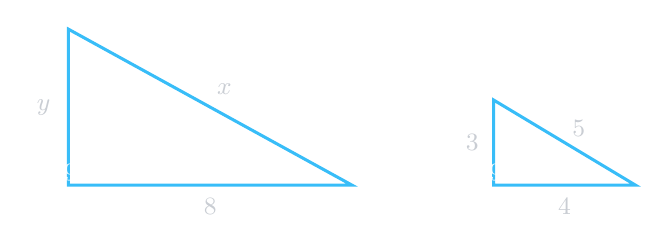
\begin{tikzpicture}[scale=0.9]
\draw[fig] (0,0)--(4,0)--(0,2.2)--cycle;
\node[dim] at (2,-0.3) {$8$};
\node[dim] at (-0.35,1.1) {$y$};
\node[dim] at (2.2,1.35) {$x$};
\node[lbl] at (0.2,0.2) {$90^\circ$};
\draw[fig] (6,0)--(8,0)--(6,1.2)--cycle;
\node[dim] at (7,-0.3) {$4$};
\node[dim] at (5.7,0.6) {$3$};
\node[dim] at (7.2,0.8) {$5$};
\node[lbl] at (6.2,0.2) {$90^\circ$};
\end{tikzpicture}
\end{center}

\textcolor{gold}{\bfseries (ii)}\\
\textcolor{green}{\bfseries Answer:} $\boxed{a=30^\circ}$.
\[
\Step{1}\; \text{Given triangles are similar and the left angle corresponds. Hence } a=30^\circ.
\]

\begin{center}
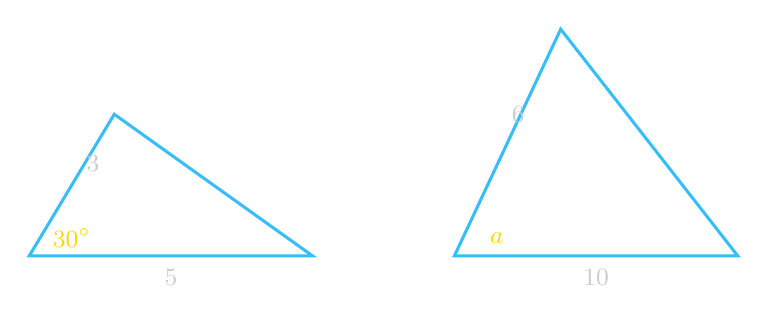
\begin{tikzpicture}[scale=0.9]
\draw[fig] (0,0)--(4,0)--(1.2,2.0)--cycle;
\node[ang] at (0.6,0.25) {$30^\circ$};
\node[dim] at (2,-0.3) {$5$};
\node[dim] at (0.9,1.3) {$3$};
\draw[fig] (6,0)--(10,0)--(7.5,3.2)--cycle;
\node[ang] at (6.6,0.25) {$a$};
\node[dim] at (8,-0.3) {$10$};
\node[dim] at (6.9,2.0) {$6$};
\end{tikzpicture}
\end{center}

\textcolor{gold}{\bfseries (iii)}\\
\textcolor{green}{\bfseries Answer:} $\boxed{x=7.5\text{ cm}}$.
\[
\begin{aligned}
\Step{1}\;& \text{Similar rectangles: }\frac{\text{height}}{\text{height}}=\frac{3}{2}=1.5.\\
\Step{2}\;& x=5(1.5)=7.5.
\end{aligned}
\]

\begin{center}
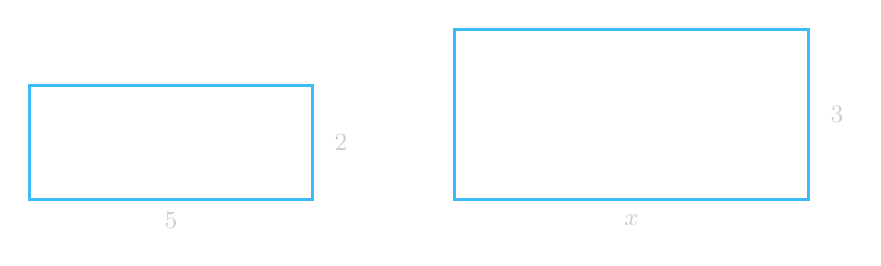
\begin{tikzpicture}[scale=0.9]
\draw[fig] (0,0)--(4,0)--(4,1.6)--(0,1.6)--cycle;
\node[dim] at (2,-0.3) {$5$};
\node[dim] at (4.4,0.8) {$2$};
\draw[fig] (6,0)--(11,0)--(11,2.4)--(6,2.4)--cycle;
\node[dim] at (8.5,-0.3) {$x$};
\node[dim] at (11.4,1.2) {$3$};
\end{tikzpicture}
\end{center}

\textcolor{gold}{\bfseries (iv)}\\
\textcolor{green}{\bfseries Answer:} $\boxed{x=2\text{ cm},\; y=3.6\text{ cm},\; z=8\text{ cm}}$.
\[
\begin{aligned}
\Step{1}\;& \text{Top bases correspond: } \frac{6}{3}=2 \Rightarrow k=2.\\
\Step{2}\;& x=\frac{4}{2}=2,\qquad y=1.8(2)=3.6,\qquad z=4(2)=8.
\end{aligned}
\]

\begin{center}
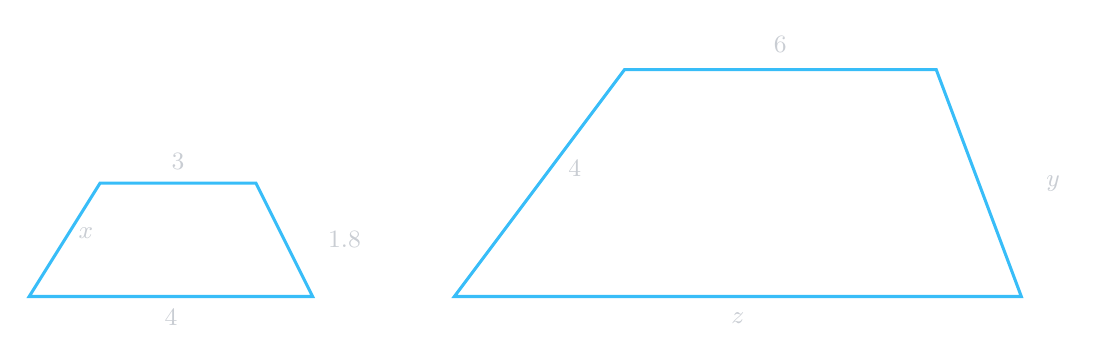
\begin{tikzpicture}[scale=0.9]
% small
\draw[fig] (0,0)--(4,0)--(3.2,1.6)--(1.0,1.6)--cycle;
\node[dim] at (2,-0.3) {$4$};
\node[dim] at (2.1,1.9) {$3$};
\node[dim] at (4.45,0.8) {$1.8$};
\node[dim] at (0.8,0.9) {$x$};
% big
\draw[fig] (6,0)--(14,0)--(12.8,3.2)--(8.4,3.2)--cycle;
\node[dim] at (10,-0.3) {$z$};
\node[dim] at (10.6,3.55) {$6$};
\node[dim] at (14.45,1.6) {$y$};
\node[dim] at (7.7,1.8) {$4$};
\end{tikzpicture}
\end{center}

\textcolor{gold}{\bfseries (v)}\\
\textcolor{green}{\bfseries Answer:} $\boxed{a=4\text{ cm},\; b=4.2\text{ cm}}$.
\[
\begin{aligned}
\Step{1}\;& \frac{6.4}{3.2}=2 \Rightarrow k=2.\\
\Step{2}\;& a=\frac{8}{2}=4,\qquad b=2.1(2)=4.2.
\end{aligned}
\]

\textcolor{gold}{\bfseries (vi)}\\
\textcolor{green}{\bfseries Answer:} $\boxed{a=4\text{ cm},\; b=6\text{ cm}}$.
\[
\begin{aligned}
\Step{1}\;& \frac{10}{5}=2 \Rightarrow k=2.\\
\Step{2}\;& a=\frac{8}{2}=4,\qquad b=3(2)=6.
\end{aligned}
\]

\textcolor{gold}{\bfseries (vii)}\\
\textcolor{green}{\bfseries Answer:} $\boxed{a=12\text{ cm}}$.
\[
\begin{aligned}
\Step{1}\;& \text{Two right triangles are similar (same acute angle at }N\text{ and right angles).}\\
\Step{2}\;& \frac{MN}{NO}=\frac{18}{12} \Rightarrow \frac{a}{8}=\frac{18}{12}=\frac{3}{2}.\\
\Step{3}\;& a=8\cdot\frac{3}{2}=12.
\end{aligned}
\]

\end{QAPair}

% ============================================================
% Q3
\begin{QAPair}{Question 3}
\textcolor{gold}{\bfseries Question:} Two triangles $ABC$ and $DEF$ are similar and
$\dfrac{AB}{DE}=\dfrac{BC}{EF}=\dfrac{CA}{FD}=2$.
If $AB=6$ cm, $BC=8$ cm, $CA=4$ cm, find the lengths of sides of $\triangle DEF$.\\
\tcblower
\textcolor{green}{\bfseries Answer:} $\boxed{DE=3\text{ cm},\; EF=4\text{ cm},\; FD=2\text{ cm}}$.
\[
\begin{aligned}
\Step{1}\;& \frac{AB}{DE}=2 \Rightarrow DE=\frac{AB}{2}=\frac{6}{2}=3.\\
\Step{2}\;& \frac{BC}{EF}=2 \Rightarrow EF=\frac{8}{2}=4.\\
\Step{3}\;& \frac{CA}{FD}=2 \Rightarrow FD=\frac{4}{2}=2.
\end{aligned}
\]

\begin{center}
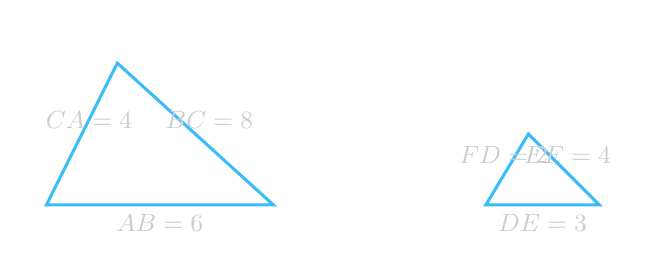
\begin{tikzpicture}[scale=0.9]
\draw[fig] (0,0)--(3.2,0)--(1.0,2.0)--cycle;
\node[lbl] at (0,-0.35) {$A$};
\node[lbl] at (3.2,-0.35) {$B$};
\node[lbl] at (1.0,2.25) {$C$};
\node[dim] at (1.6,-0.25) {$AB=6$};
\node[dim] at (2.3,1.2) {$BC=8$};
\node[dim] at (0.6,1.2) {$CA=4$};

\draw[fig] (6.2,0)--(7.8,0)--(6.8,1.0)--cycle;
\node[lbl] at (6.2,-0.35) {$D$};
\node[lbl] at (7.8,-0.35) {$E$};
\node[lbl] at (6.8,1.25) {$F$};
\node[dim] at (7.0,-0.25) {$DE=3$};
\node[dim] at (7.35,0.7) {$EF=4$};
\node[dim] at (6.45,0.7) {$FD=2$};
\end{tikzpicture}
\end{center}
\end{QAPair}

% ============================================================
% Q4
\begin{QAPair}{Question 4}
\textcolor{gold}{\bfseries Question:} Wajid noted that his shadow was $\dfrac{2}{3}$ of his height.
Find the height of a pole nearby having a shadow of $12$ m.\\
\tcblower
\textcolor{green}{\bfseries Answer:} $\boxed{18\text{ m}}$.
\[
\begin{aligned}
\Step{1}\;& \frac{\text{shadow}}{\text{height}}=\frac{2}{3}.\\
\Step{2}\;& \frac{12}{H}=\frac{2}{3}\Rightarrow H=12\cdot\frac{3}{2}=18.
\end{aligned}
\]

\begin{center}
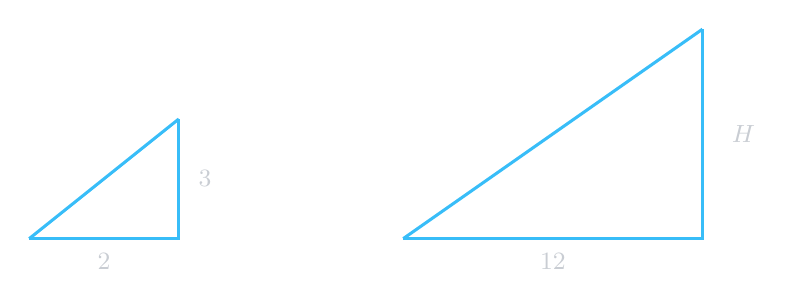
\begin{tikzpicture}[scale=0.95]
% person triangle
\draw[fig] (0,0)--(2,0)--(2,1.6);
\draw[fig] (0,0)--(2,1.6);
\node[dim] at (1,-0.3) {$2$};
\node[dim] at (2.35,0.8) {$3$};

% pole triangle
\draw[fig] (5,0)--(9,0)--(9,2.8);
\draw[fig] (5,0)--(9,2.8);
\node[dim] at (7,-0.3) {$12$};
\node[dim] at (9.55,1.4) {$H$};
\end{tikzpicture}
\end{center}
\end{QAPair}

% ============================================================
% Q5
\begin{QAPair}{Question 5}
\textcolor{gold}{\bfseries Question:} Find the length of the larger rope of the hanging bridge, where $x=y$.\\
\tcblower
\textcolor{green}{\bfseries Answer:} $\boxed{15\text{ m}}$.
\[
\begin{aligned}
\Step{1}\;& x=y \Rightarrow \text{the two triangles at the centre have equal acute angle.}\\
\Step{2}\;& \text{Both also have right angles at the walls, so triangles are similar (AA).}\\
\Step{3}\;& \frac{\text{left base}}{\text{right base}}=\frac{12}{8}=\frac{3}{2}
\Rightarrow \frac{\text{left rope}}{\text{right rope}}=\frac{3}{2}.\\
\Step{4}\;& \text{Right rope}=10\text{ m} \Rightarrow \text{left rope}=10\cdot\frac{3}{2}=15\text{ m}.
\end{aligned}
\]

\begin{center}
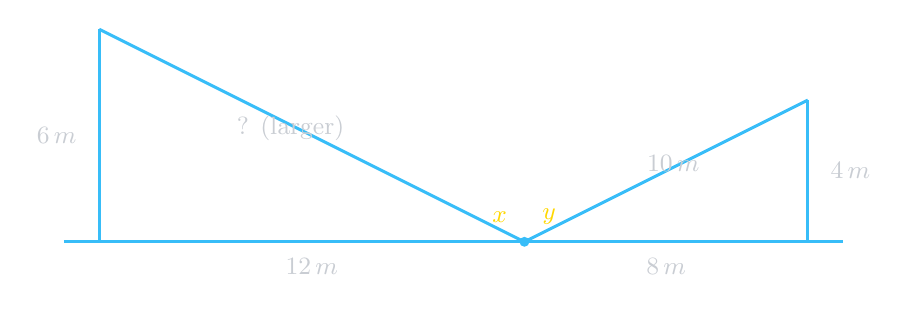
\begin{tikzpicture}[scale=0.9]
% ground
\draw[fig] (-0.5,0)--(10.5,0);
% walls
\draw[fig] (0,0)--(0,3.0);
\draw[fig] (10,0)--(10,2.0);
% center point
\coordinate (P) at (6,0);
\fill[cyan] (P) circle (2pt);

% ropes
\draw[fig] (0,3.0)--(P);
\draw[fig] (10,2.0)--(P);

\node[dim] at (-0.6,1.5) {$6\,m$};
\node[dim] at (10.6,1.0) {$4\,m$};
\node[dim] at (3.0,-0.35) {$12\,m$};
\node[dim] at (8.0,-0.35) {$8\,m$};
\node[dim] at (8.1,1.1) {$10\,m$};
\node[dim] at (2.7,1.6) {$\text{? (larger)}$};
\node[ang] at (6.35,0.35) {$y$};
\node[ang] at (5.65,0.35) {$x$};
\end{tikzpicture}
\end{center}
\end{QAPair}

% ============================================================
% Q6
\begin{QAPair}{Question 6}
\textcolor{gold}{\bfseries Question:} In the figure, $OA$ is an object lying in front of a convex lens at a distance of $10$ cm.
Find the distance of image from the lens if its size is twice that of the object.\\
\tcblower
\textcolor{green}{\bfseries Answer:} $\boxed{20\text{ cm}}$.
\[
\begin{aligned}
\Step{1}\;& m=\left|\frac{v}{u}\right|, \quad u=10\text{ cm}.\\
\Step{2}\;& \text{Image is twice the object } \Rightarrow m=2.\\
\Step{3}\;& 2=\left|\frac{v}{10}\right| \Rightarrow |v|=20 \Rightarrow \text{distance }=20\text{ cm}.
\end{aligned}
\]

\begin{center}
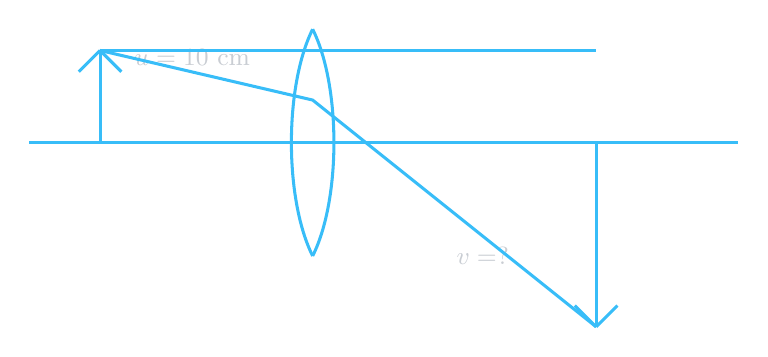
\begin{tikzpicture}[scale=0.9]
\draw[fig] (0,0)--(10,0);
% lens
\draw[fig] (4,1.6) .. controls (3.6,0.8) and (3.6,-0.8) .. (4,-1.6);
\draw[fig] (4,1.6) .. controls (4.4,0.8) and (4.4,-0.8) .. (4,-1.6);
\node[lbl] at (4,-2.1) {Lens};

% object
\draw[fig] (1,0)--(1,1.3);
\draw[fig] (1,1.3)--(0.7,1.0);
\draw[fig] (1,1.3)--(1.3,1.0);
\node[dim] at (2.3,1.2) {$u=10$ cm};

% image (twice)
\draw[fig] (8,0)--(8,-2.6);
\draw[fig] (8,-2.6)--(7.7,-2.3);
\draw[fig] (8,-2.6)--(8.3,-2.3);
\node[dim] at (6.4,-1.6) {$v=?$};

% rays (simple)
\draw[fig] (1,1.3)--(4,0.6)--(8,-2.6);
\draw[fig] (1,1.3)--(4,1.3)--(8,1.3);
\end{tikzpicture}
\end{center}
\end{QAPair}

% ============================================================
% Q7
\begin{QAPair}{Question 7}
\textcolor{gold}{\bfseries Question:} In the figure, an electricity tower is seen through the telescope.
Find the height of the tower if height of its image is $0.5$ m.\\
\tcblower
\textcolor{green}{\bfseries Answer:} $\boxed{10\text{ m}}$.
\[
\begin{aligned}
\Step{1}\;& \frac{\text{image height}}{\text{object height}}=\frac{\text{image distance}}{\text{object distance}}
\quad (\text{similar triangles}).\\
\Step{2}\;& \frac{0.5}{H}=\frac{5}{100}.\\
\Step{3}\;& H=0.5\cdot\frac{100}{5}=0.5\cdot 20=10.
\end{aligned}
\]

\begin{center}
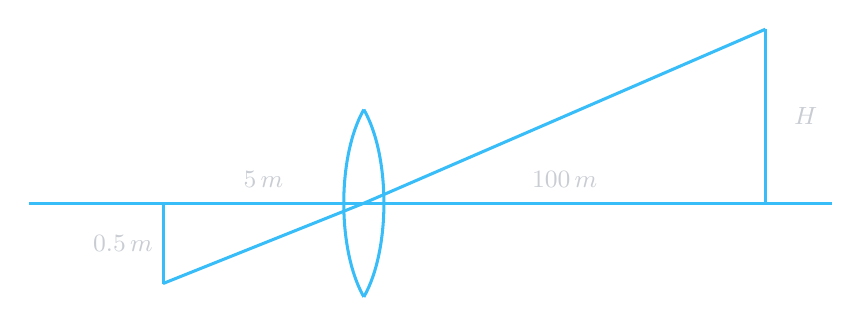
\begin{tikzpicture}[scale=0.85]
% axis
\draw[fig] (0,0)--(12,0);
% lens
\draw[fig] (5,1.4) .. controls (4.6,0.7) and (4.6,-0.7) .. (5,-1.4);
\draw[fig] (5,1.4) .. controls (5.4,0.7) and (5.4,-0.7) .. (5,-1.4);

% image on left
\draw[fig] (2,0)--(2,-1.2);
\node[dim] at (1.4,-0.6) {$0.5\,m$};
\node[dim] at (3.5,0.35) {$5\,m$};

% tower on right
\draw[fig] (11,0)--(11,2.6);
\node[dim] at (11.6,1.3) {$H$};
\node[dim] at (8.0,0.35) {$100\,m$};

% rays
\draw[fig] (2,-1.2)--(5,0)--(11,2.6);
\draw[fig] (2,0)--(5,0)--(11,0);
\end{tikzpicture}
\end{center}
\end{QAPair}

% ============================================================
% Q8
\begin{QAPair}{Question 8: Find the values of unknown quantities (all in cm)}
\textcolor{gold}{\bfseries (a) $UV \parallel YZ$}\\
\textcolor{green}{\bfseries Answer:} $\boxed{a=3}$.
\[
\begin{aligned}
\Step{1}\;& UV \parallel YZ \Rightarrow \triangle XUV \sim \triangle XYZ.\\
\Step{2}\;& \frac{XU}{XY}=\frac{XV}{XZ}. \quad XV=6,\; VZ=4 \Rightarrow XZ=10.\\
\Step{3}\;& \frac{a}{a+2}=\frac{6}{10}=\frac{3}{5}
\Rightarrow 5a=3a+6 \Rightarrow a=3.
\end{aligned}
\]

\begin{center}
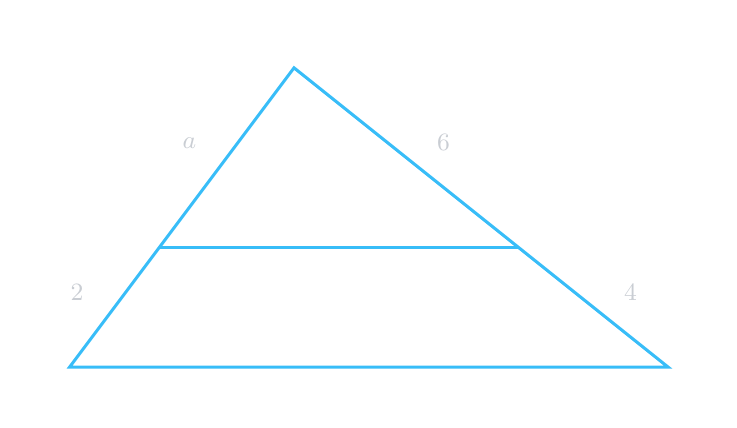
\begin{tikzpicture}[scale=0.95]
\coordinate (Y) at (0,0);
\coordinate (Z) at (8,0);
\coordinate (X) at (3,4);
\coordinate (U) at ($(X)!0.6!(Y)$);
\coordinate (V) at ($(X)!0.6!(Z)$);

\draw[fig] (Y)--(Z)--(X)--cycle;
\draw[fig] (U)--(V);

\node[lbl] at ($(X)+(0,0.3)$) {$X$};
\node[lbl] at ($(Y)+(-0.3,-0.2)$) {$Y$};
\node[lbl] at ($(Z)+(0.3,-0.2)$) {$Z$};
\node[lbl] at ($(U)+(-0.35,0)$) {$U$};
\node[lbl] at ($(V)+(0.35,0)$) {$V$};

\node[dim] at ($($(Y)!0.5!(U)$)+(-0.5,0.2)$) {$2$};
\node[dim] at ($($(U)!0.5!(X)$)+(-0.5,0.2)$) {$a$};
\node[dim] at ($($(X)!0.5!(V)$)+(0.5,0.2)$) {$6$};
\node[dim] at ($($(V)!0.5!(Z)$)+(0.5,0.2)$) {$4$};
\end{tikzpicture}
\end{center}

\textcolor{gold}{\bfseries (b) $BC \parallel DE$}\\
\textcolor{green}{\bfseries Answer:} $\boxed{y=5.25,\; x=2.4}$.
\[
\begin{aligned}
\Step{1}\;& DE \parallel BC \Rightarrow \triangle ADE \sim \triangle ABC.\\
\Step{2}\;& AB=BD+DA=5+2=7,\quad \frac{AD}{AB}=\frac{2}{7}.\\
\Step{3}\;& \frac{DE}{BC}=\frac{2}{7} \Rightarrow BC=DE\cdot\frac{7}{2}=1.5\cdot\frac{7}{2}=5.25
\Rightarrow y=5.25.\\
\Step{4}\;& \frac{AE}{AC}=\frac{2}{7},\quad AC=CE+EA=6+x,\ AE=x.\\
&\frac{x}{6+x}=\frac{2}{7}\Rightarrow 7x=12+2x\Rightarrow 5x=12\Rightarrow x=2.4.
\end{aligned}
\]

\textcolor{gold}{\bfseries (c) $AB \parallel DE$}\\
\textcolor{green}{\bfseries Answer:} $\boxed{a=16}$.
\[
\begin{aligned}
\Step{1}\;& DE \parallel AB \Rightarrow \triangle CDE \sim \triangle CBA.\\
\Step{2}\;& \frac{CE}{CB}=\frac{20}{15+20}=\frac{20}{35}=\frac{4}{7}.\\
\Step{3}\;& \frac{CD}{CA}=\frac{4}{7},\quad CA=AD+DC=12+a,\ CD=a.\\
&\frac{a}{12+a}=\frac{4}{7}\Rightarrow 7a=48+4a\Rightarrow 3a=48\Rightarrow a=16.
\end{aligned}
\]

\textcolor{gold}{\bfseries (d) $AC \parallel DE$}\\
\textcolor{green}{\bfseries Answer:} $\boxed{x=7.2,\; y=4.5}$.
\[
\begin{aligned}
\Step{1}\;& DE \parallel AC \Rightarrow \triangle BDE \sim \triangle BAC.\\
\Step{2}\;& \frac{BE}{BC}=\frac{9}{6+9}=\frac{9}{15}=\frac{3}{5}.\\
\Step{3}\;& \frac{BD}{BA}=\frac{3}{5},\ BA=AD+DB=3+y,\ BD=y.\\
&\frac{y}{3+y}=\frac{3}{5}\Rightarrow 5y=9+3y\Rightarrow y=4.5.\\
\Step{4}\;& \frac{DE}{AC}=\frac{3}{5}\Rightarrow \frac{x}{12}=\frac{3}{5}\Rightarrow x=12\cdot\frac{3}{5}=7.2.
\end{aligned}
\]
\end{QAPair}

% ============================================================
% Q9
\begin{QAPair}{Question 9}
\textcolor{gold}{\bfseries Question:} In the figure, find $\angle C$ and $\angle AED$.
Is $ED \parallel CB$?\\
\tcblower
\textcolor{green}{\bfseries Answer:} $\boxed{\angle C=50^\circ,\ \angle AED=50^\circ,\ \text{and } ED \parallel CB\ \text{(Yes).}}$
\[
\begin{aligned}
\Step{1}\;& \angle B=90^\circ,\ \angle A=40^\circ \Rightarrow \angle C=180^\circ-90^\circ-40^\circ=50^\circ.\\
\Step{2}\;& \triangle AED \text{ is right-angled at }D,\ \angle EAD=40^\circ\\
&\Rightarrow \angle AED=180^\circ-90^\circ-40^\circ=50^\circ.\\
\Step{3}\;& ED\perp AB\ \text{and}\ CB\perp AB \Rightarrow ED \parallel CB.
\end{aligned}
\]

\begin{center}
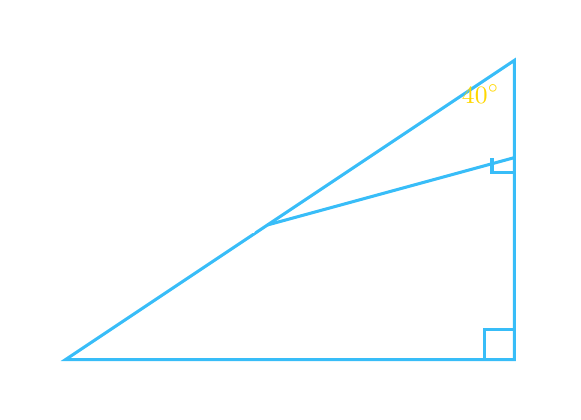
\begin{tikzpicture}[scale=0.95]
\coordinate (B) at (6,0);
\coordinate (C) at (0,0);
\coordinate (A) at (6,4);
\draw[fig] (C)--(B)--(A)--cycle;
% right angle at B
\draw[fig] (5.6,0)--(5.6,0.4)--(6,0.4);
% point D on AB
\coordinate (D) at (6,2.7);
\coordinate (E) at ($(A)!0.55!(C)$);
\draw[fig] (E)--(D);
% right angle at D (ED ⟂ AB)
\draw[fig] (6,2.5)--(5.7,2.5)--(5.7,2.7);

\node[lbl] at ($(A)+(0.25,0.2)$) {$A$};
\node[lbl] at ($(B)+(0.25,-0.2)$) {$B$};
\node[lbl] at ($(C)+(-0.25,-0.2)$) {$C$};
\node[lbl] at ($(D)+(0.25,0)$) {$D$};
\node[lbl] at ($(E)+(-0.25,0)$) {$E$};

\node[ang] at (5.55,3.55) {$40^\circ$};
\end{tikzpicture}
\end{center}
\end{QAPair}

% ============================================================
% Q10
\begin{QAPair}{Question 10}
\textcolor{gold}{\bfseries Question:} In the figure, $\triangle XYZ$ is an equilateral triangle and $LM \parallel YZ$.
Find measures of $a$ and $b$. What type of triangle is $XLM$ with respect to sides and angles?\\
\tcblower
\textcolor{green}{\bfseries Answer:} $\boxed{a=60^\circ,\ b=60^\circ,\ \triangle XLM\text{ is equilateral (all sides equal, all angles }60^\circ\text{).}}$
\[
\begin{aligned}
\Step{1}\;& \triangle XYZ \text{ equilateral} \Rightarrow \angle X=\angle Y=\angle Z=60^\circ.\\
\Step{2}\;& LM \parallel YZ \Rightarrow \triangle XLM \sim \triangle XYZ\ (\text{AA}).\\
\Step{3}\;& \Rightarrow \angle XLM=a=60^\circ,\ \angle XML=b=60^\circ.\\
\Step{4}\;& \text{So }\triangle XLM \text{ has all angles }60^\circ \Rightarrow \text{equilateral.}
\end{aligned}
\]

\begin{center}
\begin{tikzpicture}[scale=0.95]
\coordinate (Y) at (0,0);
\coordinate (Z) at (8,0);
\coordinate (X) at (4,6.5);
\coordinate (L) at ($(X)!0.55!(Y)$);
\coordinate (M) at ($(X)!0.55!(Z)$);
\draw[fig] (Y)--(Z)--(X)--cycle;
\draw[fig] (L)--(M);

\node[lbl] at ($(X)+(0,0.3)$) {$X$};
\node[lbl] at ($(Y)+(-0.3,-0.2)$) {$Y$};
\node[lbl] at ($(Z)+(0.3,-0.2)$) {$Z$};
\node[lbl] at ($(L)+(-0.25,0)$) {$L$};
\node[lbl] at ($(M)+(0.25,0)$) {$M$};

\node[ang] at ($(L)+(0.35,0.35)$) {$a$};
\node[ang] at ($(M)+(-0.35,0.35)$) {$b$};
\end{tikzpicture}
\end{center}
\end{QAPair}

% ============================================================
% Q11
\begin{QAPair}{Question 11}
\textcolor{gold}{\bfseries Question:} Find the height of the shorter tree if the longer one is $12$ m high.
The observer is at a distance of $25$ m from the shorter tree and the distance between both trees is $5$ m.\\
\tcblower
\textcolor{green}{\bfseries Answer:} $\boxed{10\text{ m}}$.
\[
\begin{aligned}
\Step{1}\;& \text{Distance from observer to taller tree}=25+5=30\text{ m}.\\
\Step{2}\;& \text{Line of sight makes similar triangles: }\frac{h}{12}=\frac{25}{30}.\\
\Step{3}\;& h=12\cdot\frac{25}{30}=12\cdot\frac{5}{6}=10.
\end{aligned}
\]

\begin{center}
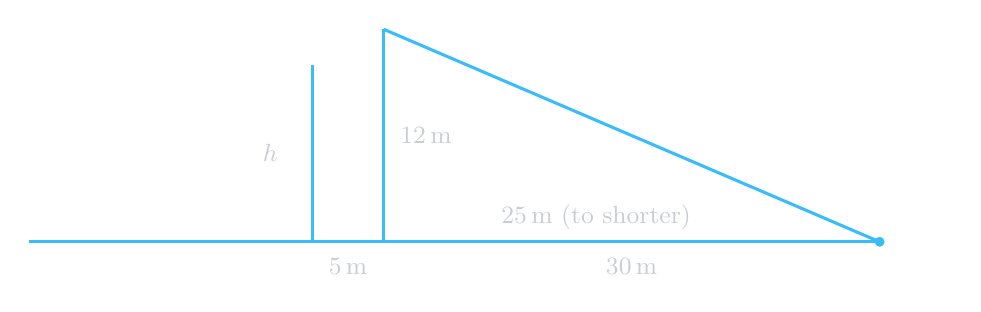
\begin{tikzpicture}[scale=0.9]
% ground line
\draw[fig] (0,0)--(12,0);
% shorter tree at x=4
\draw[fig] (4,0)--(4,2.5);
\node[dim] at (3.4,1.25) {$h$};
% taller tree at x=5
\draw[fig] (5,0)--(5,3.0);
\node[dim] at (5.6,1.5) {$12\,\text{m}$};

% observer at x=12
\fill[cyan] (12,0) circle (2pt);
\node[lbl] at (12.2,-0.25) {Observer};

% sight line from top of tall to observer passing near top of short
\draw[fig] (5,3.0)--(12,0);

% distances
\node[dim] at (8.5,-0.35) {$30\,\text{m}$};
\node[dim] at (8.0,0.35) {$25\,\text{m (to shorter)}$};
\node[dim] at (4.5,-0.35) {$5\,\text{m}$};
\end{tikzpicture}
\end{center}
\end{QAPair}

\end{document}